\section{球面镜}\label{sec:1-4}

实际上还常常用到\textbf{球面镜},它的反射面是球面的一部分。球面镜有两种,
  一种是用球面的里面做反射面的,叫做\textbf{凹镜};
另一种是用球面的外面做反射面的,叫做\textbf{凸镜}。

把凹镜对着太阳,太阳的平行光被凹镜反射后,就会聚在一点 $F$(图 \ref{fig:1-10})。
如果把一块小纸片放在这一点,小纸片上就出现一个明亮的点。过一会儿,
亮点处的纸就被烧焦。这一点就叫做凹镜的\textbf{焦点}。

利用凹镜能把太阳光会聚在焦点的性质,可以制成煮饭、烧水用的太阳灶和给蒸汽轮机
生产水蒸气或者熔化难熔物质的太阳炉。需要加热的物体就放在凹镜的焦点处。
凹镜的面积越大,能够会聚的太阳光就越多,焦点处的温度就越高。
\hyperref[fig:pic2]{彩图2} 所示的是太阳能焊接机。
它的凹镜的直径为 2.5 米,焦点处的温度可达 $2000\celsius$,能使金属熔化,进行焊接。

\begin{figure}[htbp]
    \centering
    \begin{minipage}{7cm}
    \centering
    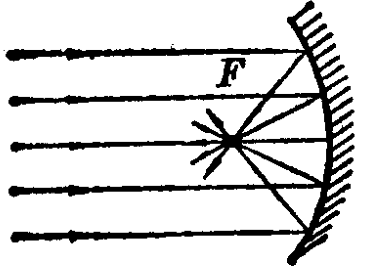
\includegraphics[width=5cm]{../pic/czwl2-ch1-10}
    \caption{凹镜能使平行光\\会聚在焦点上}\label{fig:1-10}
    \end{minipage}
    \qquad
    \begin{minipage}{7cm}
    \centering
    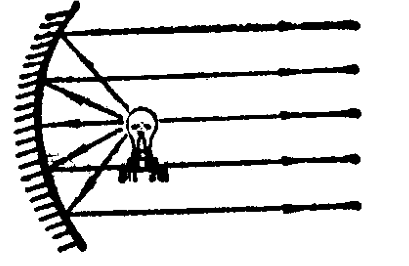
\includegraphics[width=5cm]{../pic/czwl2-ch1-11}
    \caption{从凹镜焦点发出的光\\被反射后平行射出}\label{fig:1-11}
    \end{minipage}
\end{figure}


如果把光源放在凹镜的焦点上,光源发出的光被凹镜反射以后,将成为平行光(图 \ref{fig:1-11})。
汽车头灯(图 \ref{fig:1-12})就是利用凹镜的这种性质做成的。汽车头灯是双光灯,它有两个灯丝:
一个是远距光灯丝,在凹镜的焦点上,发出的光经凹镜反射后集中向前方平行射出,照亮远处的道路;
另一个是近距光灯丝,不在凹镜的焦点上,发出的光经凹镜反射后只照亮车前不远的地方,
可以避免使对面开来的汽车司机感到刺眼。

\begin{figure}[htbp]
    \centering
    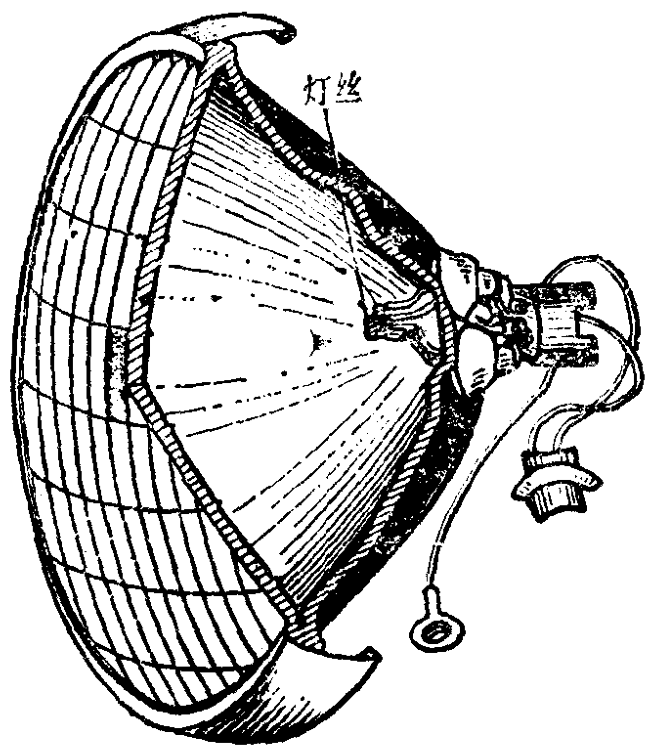
\includegraphics[width=0.5\textwidth]{../pic/czwl2-ch1-12}
    \caption{汽车头灯}\label{fig:1-12}
\end{figure}


凸镜对于光起发散作用。射到凸镜上的平行光,经凸镜反射后不能会聚于一点,而是变得发散(图 \ref{fig:1-13})。

\begin{figure}[htbp]
    \centering
    \begin{minipage}{7cm}
    \centering
    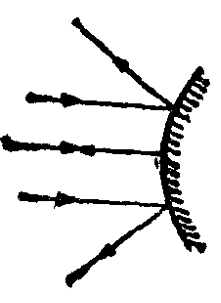
\includegraphics[width=4cm]{../pic/czwl2-ch1-13}
    \caption{凸镜能使平行光发散}\label{fig:1-13}
    \end{minipage}
    \qquad
    \begin{minipage}{7cm}
    \centering
    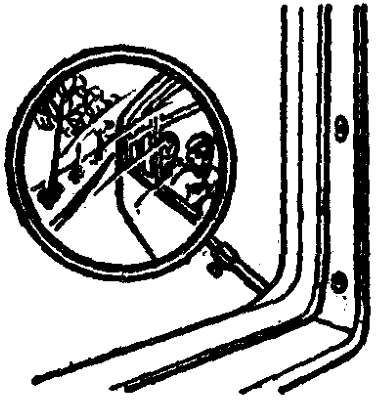
\includegraphics[width=6cm]{../pic/czwl2-ch1-14}
    \caption{汽车上的观后镜}\label{fig:1-14}
    \end{minipage}
\end{figure}

汽车驾驶室外面的观后镜常用凸镜(图 \ref{fig:1-14})。为什么用凸镜而不用平面镜呢?
从图 \ref{fig:1-15} 中可以看出,对于口径相同的平面镜和凸镜来说,当人离镜同样远时,
从凸镜观察到的范围要比平面镜大。
\begin{figure}[htbp]
    \centering
    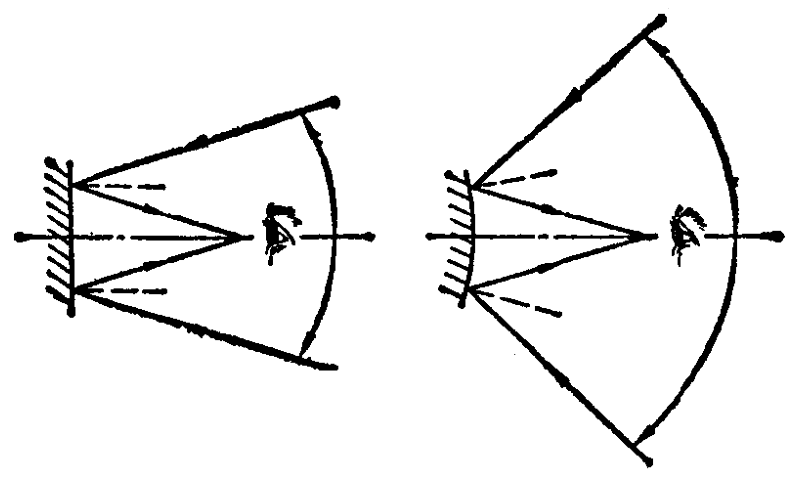
\includegraphics[width=0.6\textwidth]{../pic/czwl2-ch1-15}
    \caption{}\label{fig:1-15}
\end{figure}
汽车上用凸镜做观后镜,可以使司机从镜中观察到车后侧较大范围内的物体,保证行车安全。
有的城市在马路交叉处和拐弯处也常常安装一个大的凸镜,
使交通民警和行人以看到较大范围的车辆行驶情况,保证交通安全。


\lianxi

(1) 入射光线跟镜面的夹角是 $25^\circ$,入射光线跟反射光线的夹角是多少?

(2) 要想使反射光线跟入射光线成直角,入射角应当是多大?
如果使入射光线逐渐靠拢法线,反射光线的方向怎样变化?

(3) 在黑喑的房子里,桌子上立着一平面镜,镜子后面是白色的墙。
用手电筒正对着镜子和墙照射,从旁边看时,会发现墙被照亮了,而镜子却显得很暗〈图 \ref{fig:1-16})。
实际做做看,并说明为什么墙反而比镜子亮。

\begin{figure}[htbp]
    \centering
    \begin{minipage}{7cm}
    \centering
    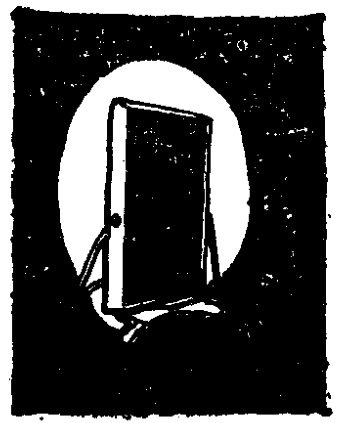
\includegraphics[width=5cm]{../pic/czwl2-ch1-16}
    \caption{}\label{fig:1-16}
    \end{minipage}
    \qquad
    \begin{minipage}{7cm}
    \centering
    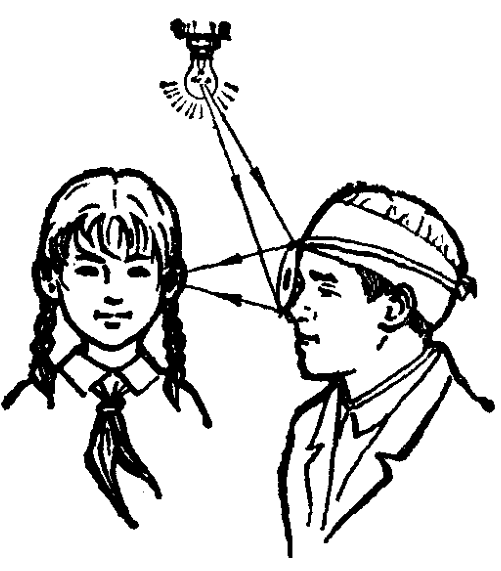
\includegraphics[width=5cm]{../pic/czwl2-ch1-17}
    \caption{}\label{fig:1-17}
    \end{minipage}
\end{figure}

(4) 一人立于平面镜前 1 米处,这个人在镜子里的像离他本人多远?
如果人向镜面前进 0.5 米,人和像间的距离又是多少?

(5) 医生检查耳道时,为什么常戴一个凹镜(图 \ref{fig:1-17})。


